%!TEX program = xelatex
% 完整编译: xelatex -> bibtex -> xelatex -> xelatex
\documentclass[lang=cn,11pt,a4paper]{paper}

\title{地方补贴式租赁住房的挤出效应:来自LIHTC计划的新证据}
\author{Michael D. Eriksen\thanks{\href{http://www.eriksen.myweb.uga.edu}{迈克尔·D·埃里克森},电话:+1 706 542 9774,传真:+1 706 542 4295,电子邮件:\email{eriksen@terry.uga.edu}。佐治亚大学特里商学院房地产系,美国乔治亚州雅典城,GA 30602。} \and Stuart S. Rosenthal\thanks{\href{http://www.faculty.maxwell.syr.edu/rosenthal}{斯图亚特·S·罗森塔尔},通讯作者,电话:+1 315 443 3809,传真:+1 315 443 1081,电子邮件:\email{ssrosent@maxwell.syr.edu}。锡拉丘兹大学经济系和政策研究中心,美国纽约锡拉丘兹,13244-1020。}\; \thanks{\href{https://www.sciencedirect.com/science/article/pii/S0047272710000885}{英文原文链接}。作者非常感谢约翰·D·凯瑟琳·麦克阿瑟基金会,福特基金会以及住房和城市发展部为该项目提供的资金。本文从许多个人的有益评论中受益。我们感谢两位匿名编辑Dennis Epple(编辑),Denise DiPasquale,Gary Engelhardt,Jeffrey Kubik,Edgar Olsen,Erika Poethig,Steve Ross,Michael Stegman,Bruce Weinberg,Johnny Yinger,以及参加2007年1月AREUEA会议和俄亥俄州立大学提供有用的意见。当然,文责自负。}}
\translator{翻译者:\href{https://tomben.me/}{任\ 涛}}

%\version{0.08}
\date{\zhtoday}

\begin{document}

\maketitle

\begin{abstract}
  \hspace{2\ccwd}自1987年成立以来,低收入住房税收抵免(LIHTC)计划已迅速发展成为美国有史以来最大的低收入住房补贴建筑来源,占最近所有多户出租建筑的三分之一。本文研究了这种日益重要的中低收入住房来源的挤出效应。为此,我们分析了LIHTC建设对地理的三个不同层次(MSA,县和10英里半径圆)的影响。这使我们能够采用越来越广泛的地域固定效应,以帮助区别未观察到的因素。政治变量也被用作进一步促进识别的工具。
  
  \!在我们所有的模型中,IV估计产生的拥挤要比OLS大得多,这证实了LIHTC开发对新建筑成熟区域的内生吸引力。我们最可靠的IV估算表明,LIHTC发展的近100\%被 新建的无补贴租赁单位的数量,尽管这一点估计值附近的置信区间允许进行不太剧烈的评估。其他估算表明,LIHTC的发展对自住房建设的影响要小得多,但这些估算并不精确。总体而言,尽管LIHTC的发展可能会很好地影响低收入公寓的位置,但我们的估计表明,该计划对新开发的出租房屋数量的影响似乎很小。

  \keywords{挤出效应,保障性住房,LIHTC}
\end{abstract}
\vspace{10pt}

\begin{tcolorbox}[
	colback=yellow!10!white,
  colframe=red!30!black,
  fontupper = \itshape,
]
“I rise today to introduce the Affordable Housing Tax Credit Enhancement Act of 2005. … the bill would double the current LIHTC [annual allocations], which would yield twice the number of affordable units annually. … Today, the LIHTC program is widely regarded as the nation's most successful housing production program resulting in the construction and rehabilitation of more than 1.3 million housing units for lower income households. …”
\vspace{5pt}

\textbf{Statements Submitted to Congressional Record: May 26, 2005 By Rep. William Jefferson (D-LA)}

\tcblower

“我今天起草来介绍《2005年经济适用房税收抵免增强法案》。……该法案将使目前的LIHTC(年度拨款)翻一番,这将使每年的经济适用房数量增加一倍。 …今天,LIHTC计划被公认为是美国最成功的住房生产计划,它为低收入家庭建造和修复了130万套住房……”
\vspace{5pt}

\textbf{众议员William Jefferson(D-LA)在2005年5月26日提交国会记录的声明。}

\end{tcolorbox}
\vspace{10pt}

\section{引言}

提供给穷人的住房援助的方式仍然有很多甚至是激烈的争论:政府应该通过需求方优惠券类型计划(例如第8节优惠券)还是通过公共和低价等供应方建筑补贴在地方投资人 收入住房税收抵免(LIHTC)住房? 在此背景下,本文考察了快速增长的LIHTC计划,并强调了LIHTC建设在多大程度上排除了无偿租赁房屋的开发。 一些进一步的背景将有助于使LIHTC计划成为现实。

在1930年代末至1980年代中期,联邦政府通过“传统”公共住房计划建造了超过一百万套住房。 重要的是,这些计划通常将入住人数限制在贫困线以下或以下的家庭 \citep{Olsen2003365}\,\footnote{\cite{Olsen2003365}指出,至少有29种不同的公共住房计划。 这些项目中的家庭通常将其总收入的30\%用于租金。}。到1980年代,至少在两个方面,人们的担忧开始削弱对公共住房进一步扩大的支持。 首先是政府建设,拥有和运营公共住房项目。 关于某些活动是否最好留给私营部门存在一些基本问题。 第二个是公共住房项目造成了密集的贫困集群,加剧了人们对犯罪,邻里衰落以及对项目中儿童成长的不利影响的担忧(例如,可参见 \cite{Currie200099,Jencks1990111})。出于这些原因,公共住房的建设在1980年代初结束了,1990年代开始拆除性能最差的项目\,\footnote{在某些情况下,例如根据HOPE VI计划,公共住房结构进行了改建,但在大多数情况下,通常向住户发放住房券,并告知他们私下寻求住房 \cite{Jacob2004233}。}。

随着1986年的税收改革法案(TRA86),低收入住房税收抵免(LIHTC)计划应运而生,作为公共住房的替代方案,同时也抵消了改革对出租住房业主的其他税收优惠的取消\citep{USCongress1987}\,\footnote{根据美国税法第42条,LIHTC计划由国内税收署管理。}。LIHTC项目的前提与公共住房明显不同,它是基于政府和营利性开发商之间的合作关系。根据LIHTC的规定,私人市场开发商可以从非土地建设成本中获得高额补贴,补贴的慷慨程度还会随着LIHTC为收入低于住房和城市发展部(HUD)规定标准的租户保留的公寓份额的增加而增加\,\footnote{联邦政府通过一项为期10年的年度不可退还的联邦所得税抵免,一美元一美元地降低私人开发商的联邦所得税责任,补贴私人开发商30 - 91\%的非土地建设成本 \cite{Eriksen2009141}。由于补贴的慷慨程度随着分配给低收入居民的项目单元份额的增加而增加,大多数开发商的应对措施是让所有单元都住满符合收入标准的租户。不遵守LIHTC的操作规则将导致开发商丧失未来的税收抵免,并偿还1/10。}。此外,开发商同意在至少15年内,将目标公寓的租金设定在规定的上限以下,之后才允许收取市场租金。考虑到这些规定,LIHTC在某些方面是一种有针对性的租金控制形式,其中资格规则限制占用。

LIHTC很快就超越了之前所有基于场所的补贴租赁项目,成为美国历史上最大的此类项目。在\tabref{tab1}中,值得注意的是,从1987年到2006年,大约建造了160万套LIHTC住房,占最近建造的多户出租住房的大约三分之一。\figref{fig1}进一步说明了这一点。这个数字显示了过去60年公共住房的建设和LIHTC的发展\,\footnote{用于创建\figref{fig1}的公共住房数据是从住房和城市发展部的分析师那里获得的,并得到了约翰·麦克阿瑟和凯瑟琳·麦克阿瑟以及阿布特协会的帮助。这些数据在两个方面不同于 \url{http://www.huduser.org} 的公开数据。首先,我们的数据包含每个“项目”从1937年到2000年投入使用的年份。这使我们能够代表每十年新建的公共住房。此外,我们的数据还包括1990年代拆除公共住房的信息。LIHTC数据是从 \url{http://www.lihtc.huduser.org} 的平显获得的。}。最近LIHTC发展的繁荣是显而易见的。同样显而易见的是,在\tabref{tab2}中,请注意,尽管LIHTC计划的成本相对于住房券计划来说似乎不算高,但LIHTC计划的绝对成本却很高。2006年,住房代金券项目耗资近210亿美元。相比之下,与LIHTC计划相关的联邦税收损失总计49亿美元。然而,由于从2001年开始分配的信贷增加了40\%,预计这一费用在未来几年将急剧增加\,\footnote{即使最近有关扩大LIHTC项目的提议尚未出台,这些增长也会发生。有关各种形式的低收入者住房支助费用的详细资料载于住房和城乡建设局的一份报告 \cite{USCongress2005}。}。


\begin{table}[h]
\centering
\setlength{\tabcolsep}{12mm}
  \begin{threeparttable}
  \caption{国家LIHTC汇总统计\tnote{a}}\label{tab1}
    \begin{tabular}{ccc}
  \toprule
  & 年度拨款总额 (\$)\tnote{b}
  & 补贴单位数量\tnote{c} \\
  \midrule
  1987 & 980,533,493 & 34,491 \\
  1988 & 3,140,987,971 & 81,408 \\
  1989 & 4,387,952,511 & 126,200 \\
  1990 & 2,888,647,156 & 74,029 \\
  1991 & 5,207,469,242 & 111,970 \\
  1992 & 4,255,013,370 & 91,300 \\
  1993 & 5,205,992,598 & 103,756 \\
  1994 & 5,915,192,114 & 117,099 \\
  1995 & 4,892,206,044 & 86,343 \\
  1996 & 4,277,723,133 & 77,003 \\
  1997 & 4,225,625,522 & 70,453 \\
  1998 & 3,999,808,231 & 67,822 \\
  1999 & 3,983,473,499 & 62,240 \\
  2000 & 3,895,882,268 & 59,601 \\
  2001 & 4,624,992,306 & 67,261 \\
  2002 & 5,162,994,677 & 69,310 \\
  2003 & 5,507,541,467 & 73,877 \\
  2004 & 5,680,347,051 & 75,600 \\
  2005 & 5,556,042,690 & 70,630 \\
  2006 & 6,668,538,964 & 74,278 \\
  总计 & 90,456,964,308 & 1,594,671 \\
  \bottomrule
    \end{tabular}
  \begin{tablenotes}
    \footnotesize
    \item[a] 数据由国家住房当局全国委员会汇编。
    \item[b] 计算时假设通货膨胀率为3\%,并且在分配后的10年内将申请已分配的税收抵免。
    \item[c] 不包括未补贴的市场价格单位,有时包括在LIHTC补贴的房产中。
  \end{tablenotes}
\end{threeparttable}
\end{table}

\begin{figure}[h]
	\centering
	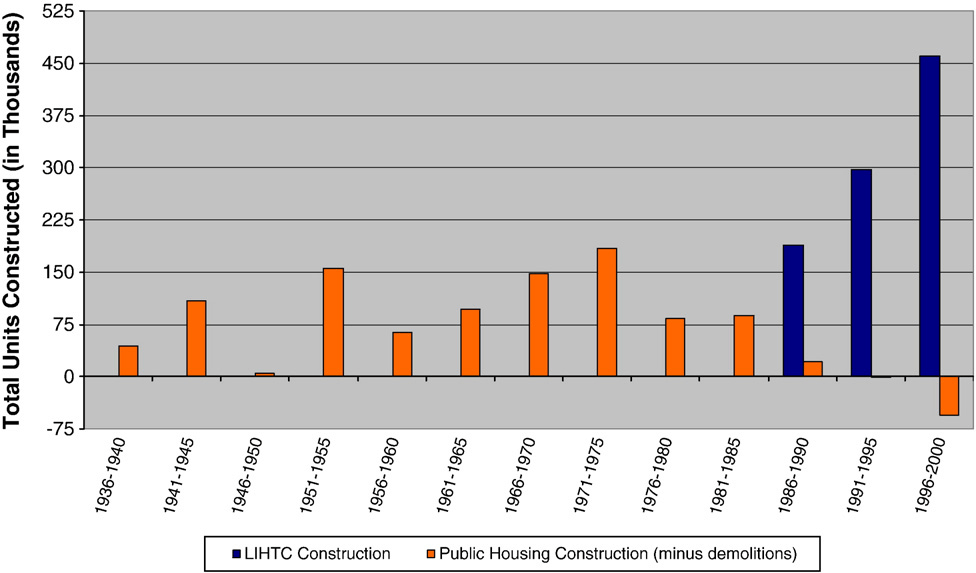
\includegraphics[width=13cm]{fig1.png}
	\caption{基于地点的住房补贴建造和拆除}\label{fig1}
\end{figure}

很明显,LIHTC是一个昂贵的项目。同样明显的是,LIHTC是一种有针对性的租金控制形式。不太明显的是,LIHTC的目标实际上是温和的,而不是低收入的租户。在考虑LIHTC计划的挤出效应时,这一点尤其重要,无论是在总体上还是在公共住房方面。尽管私营部门很少为接近或低于贫困线的家庭建造无补贴住房,但它经常建造中等收入的出租住房。这表明,虽然建造公共住房只是间接地与未受资助的私人开发项目竞争,但LIHTC项目与未受资助的建筑项目直接竞争。因为排挤是在政府与私营部门争夺市场份额时出现的,所以以中等收入家庭为目标增加了LIHTC项目取代无补贴开发的可能性。鉴于LIHTC计划的这一特点的重要性,我们在下面提供了四条证据,证实LIHTC倾向于以收入远高于传统公共住房的家庭为目标。

首先要考虑的一点是,LIHTC补贴住房的租金上限定得相对较高。准确地说,租金上限设定为家庭收入中位数,即生活津贴中位数)的18\%,每年由住房和城市发展部规定\,\footnote{之所以提出18\%的AMI收入门槛,是因为补贴单元的居住者的收入必须低于AMI的60\%,而向补贴单元的个人收取的租金不得超过该上限的30\%。}。尽管租金上限因城市而异,但它们与住房和城市发展部规定的公平市场租金想尽相近 \citep{Cummings1999257},后者用于管理第8节凭证领取者支付的租金。这些租金通常在上年私人市场合同租金的40\%至50\%之间。对于许多低收入家庭来说,这种水平的租金是负担不起的。

第二点也是相关的一点是,LIHTC补贴住房租户的收入限制也定在相对较高的水平。具体而言,住房和城市发展部将LIHTC补贴单位的收入资格定为最低收入水平的60\%。这一限额远远高于传统公共住房开发居住者的收入限额\,\footnote{例如,在2000年的华盛顿州DC市生活津贴中,住房和城市发展部为一个三口之家规定的LIHTC收入限额为43,500加元(大约相当于该规模家庭家庭收入中位数的60\%)。LIHTC项目业主在那一年可以向这样一个家庭收取的最高租金是每月1088美元。相比之下,2000年华盛顿州DC市的所有出租单元(未补贴加补贴单元)的租金中位数为每月840美元。参见住房和城市发展部网站:\url{http://www.huduser.org}。}。


%\nocite{*}
\bibliography{ref}

\appendix
\appendixpage
\addappheadtotoc
\section{How I became inspired}


\end{document}
